La desintegración en cadena  del $^{235} U$ se conoce como la serie del actínido \cite{Podgorsak.2016}. Como parte del proceso de desintegración radiactiva, los productos de fisión del uranio emiten neutrones y rayos gamma al atravesar una serie de decaimientos beta \cite{Guo.2016}. La causa de esta serie de desintegraciones nucleares se debe a la razón de neutrones sobre protones, es mediante el canal beta que estos núcleos logran la estabilidad \cite{Guo.2016}. 

De acuerdo con \textit{Guo et al} en \cite{Guo.2016}, al momento de analizar una cadena de desintegración compleja se simplifica el problema al resolver la reacción a través de reacciones lineales en las que cada núcleo está relacionado solo a un núcleo madre; el núcleo madre puede estar en su estado base o en un estado excitado, partiendo de esto llamamos a cada cadena lineal \textit{la del estado base} y \textit{la del estado excitado}, respectivamente.

El proceso de desintegración del uranio-235 contempla bifurcaciones en varios puntos, esto es: hay productos de desintegración que pueden a su vez producir uno de dos posibles núcleos más estables \cite{HUBENER2003211, International_Atomic_Energy_Agency2013-bq}. La literatura observa más o menos bifurcaciones para el proceso, como podemos apreciar en \cite{HUBENER2003211,International_Atomic_Energy_Agency2013-bq,Pratiwi.2021,Loch.2013}, por mencionar tres ejemplos. Para mantener la simulación lo más fiel posible al proceso real, tomamos como referencia la cadena presentada por \textit{Hübener} en \cite{HUBENER2003211}, la cual está ilustrada en la imagen \ref{cadenadelu235}.

\begin{figure}[H]
    \centering
    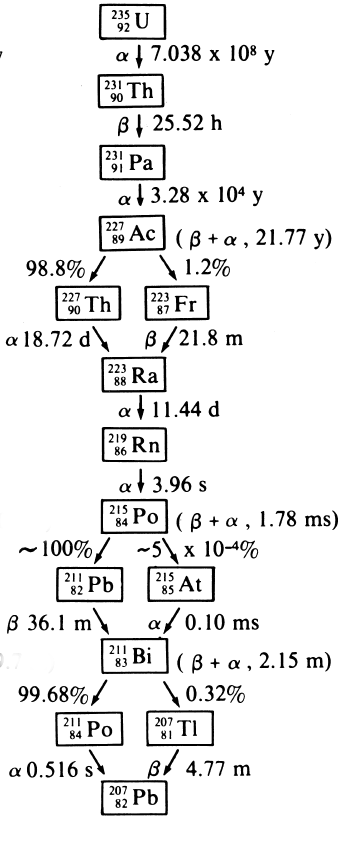
\includegraphics[scale=0.425]{imagenes/cadenaluz.png}
    \caption{Cadena de desintegración del U235 hasta Pb207. Tomada de \cite{HUBENER2003211}}.
    \label{cadenadelu235}
\end{figure}

Contemplar el proceso de enriquecimiento del material fisionable complica en gran manera la resolución del problema, es por esto que ignoraremos esta etapa del proceso.  

\subsection{Ecuaciones de Bateman para la serie del actínido}

Es posible modelar las ecuaciones de Bateman en una notación matricial contemplando un sistema de ecuaciones para cada posible bifurcación \cite{Pratiwi.2021}. Nuestra intención en este estudio es más bien contemplar las bifurcaciones mediante un modelo diferencial estocástico.

Tomando en cuenta las condiciones iniciales \ref{condicioninicialpadre} y \ref{condicioninicialproductos} y la forma de $N_i(t)$ en \ref{iesimonucleo}, podemos plantear las ecuaciones de Bateman de la siguiente forma:
\begin{align}
    N_1'(t)&=-\lambda_1 N_1(t)\\ \label{ecubateman1}
    N_2'(t)&=\lambda_1 N_1(t) -\lambda_2 N_2(t)\\
    N_3'(t)&=\lambda_2 N_2(t) -\lambda_3 N_3(t)\\
    N_4'(t)&=\lambda_3 N_3(t) -\lambda_4 N_4(t)\\
    N_5'(t)&=(1-f_4)\lambda_4 N_4(t) -\lambda_5 N_5(t)\\
    N_6'(t)&=f_4 \lambda_4 N_4(t) -\lambda_6 N_6(t)\\
    N_7'(t)&=\lambda_6 N_6(t) + \lambda_5 N_5(t) -\lambda_7 N_7(t)\\
    N_8'(t)&=\lambda_7 N_7(t) -\lambda_8 N_8(t)\\
    N_9'(t)&=\lambda_8 N_8(t) -\lambda_9 N_9(t)\\
    N_{10}'(t)&=\lambda_9 N_9(t) -\lambda_{10} N_{10}(t)\\
%\end{align}
%
%\begin{align}
    N_{11}'(t)&=\lambda_{10} N_{10}(t) -\lambda_{11} N_{11}(t)\\
    N_{12}'(t)&=(1-f_{11})\lambda_{11} N_{11}(t) -\lambda_{12} N_{12}(t)\\
    N_{13}'(t)&=f_{11}\lambda_{11}N_{11}(t) -\lambda_{13} N_{13}(t)\\
    N_{14}'(t)&=\lambda_{12} N_{12}(t) + \lambda_{13} N_{13}(t)
    \label{ecubateman14}
\end{align}

\noindent donde $f_k$ son tasas de ramificación. Las $N_i(t)$ se definen de la siguiente manera:
\begin{itemize}
    \item $N_1(t)\equiv$ \textit{Núcleos de} $^{235}U$.
    \item $N_2(t)\equiv$ \textit{Núcleos de} $^{231}Th$.
    \item $N_3(t)\equiv$ \textit{Núcleos de} $^{231}Pa$.
    \item $N_4(t)\equiv$ \textit{Núcleos de} $^{227}Ac$.
    \item $N_5(t)\equiv$ \textit{Núcleos de} $^{227}Th$
    \item $N_6(t)\equiv$ \textit{Núcleos de} $^{223}Fr$
    \item $N_7(t)\equiv$ \textit{Núcleos de} $^{223}Ra$.
    \item $N_8(t)\equiv$ \textit{Núcleos de} $^{219}Rn$.
    \item $N_9(t)\equiv$ \textit{Núcleos de} $^{215}Po$.
    \item $N_{10}(t)\equiv$ \textit{Núcleos de} $^{211}Pb$
    \item $N_{11}(t)\equiv$ \textit{Núcleos de} $^{211}Bi$.
    \item $N_{12}(t)\equiv$ \textit{Núcleos de} $^{211}Po$
    \item $N_{13}(t)\equiv$ \textit{Núcleos de} $^{207}Tl$.
    \item $N_{14}(t)\equiv$ \textit{Núcleos de} $^{207}Pb$
\end{itemize}

\noindent para los factores de ramificación tenemos:
\begin{itemize}
    \item $f_4=\frac{\lambda_{4,\alpha}}{\lambda_{4,\alpha}+\lambda_{4,\beta}}$, donde $\lambda_{4,\alpha}$ es la tasa de desintegración del $^{227}Ac$ hacia $^{223}Fr$, mientras que $\lambda_{4,\beta}$ representa la tasa de desintegración de $^{227}Ac$ hacia $^{227}Th$. 
    \item $f_{11}=\frac{\lambda_{11,\alpha}}{\lambda_{11,\alpha}+\lambda_{11,\beta}}$, donde $\lambda_{11,\alpha}$ es la tasa de desintegración del $^{211} Bi$ hacia $^{207} Tl$, mientras que $\lambda_{11,\beta}$ representa la tasa de desintegración de $^{211} Bi$ hacia $^{211} Po$.
\end{itemize}

Para obtener las tasas de ramificación es preciso conocer los valores de las constantes de decaimiento en cada canal del radionúclido. Si conocemos la probabilidad de desintegración mediante un canal dado y la vida media del radionúclido, es posible calcular $\lambda_{i,\alpha}$ y $\lambda_{i,\beta}$ para el iésimo núcleo con:

$$\lambda_{i,canal}=\frac{\textrm{Probablidad del canal}}{\tau_i}$$

De acuerdo con los archivos de \textit{National Nuclear Data Center}, las probabilidades para el canal alfa y el beta en el Ac-227 son, respectivamente, 0.0138 y 0.9862. Las probabilidades para el canal alfa y el beta en el Bi-211 son, respectivamente, 0.99724 y 0.00276. De manera que $f_4=0.01380$ y $f_{11}=0.99724$.

La constante de decaimiento $\lambda_i$ para el i-ésimo núcleo es una función del período de semidesintegración $T_{1/2}^{(i)}$, estos valores son conocidos y están documentados en la literatura, tal es el caso de \cite{Flanagan1954}. La tabla \ref{tabladeconstantesdedesintegracion} muestra las constantes de decaimiento de cada núcleo en las ecuaciones \ref{ecubateman1} hasta \ref{ecubateman14} junto con el período de semidesintegración que le concierne según estos registros. 

%\begin{minipage}{\textwidth}
%\begin{table}[h]
%    \centering
\begin{center}
\noindent\begin{tabular}{|c|l|l|}
\hline
Radionúclido & \multicolumn{1}{c|}{$T_{1/2}$} & \multicolumn{1}{c|}{$\lambda\ (a^{-1})$} \\\hline\hline 
$^{235}U$ & $7.13\times10^8$ a & $9.7216\times 10^{-10}$ \\
$^{231}Th$ & 26.64 h & $2.2793\times 10^{2}$ \\
$^{231}Pa$ & 34 300 a & $2.0208\times 10^{-5}$ \\
$^{227}Ac$ & 22.0 a & $3.1507\times 10^{-2}$ \\
$^{227}Th$ & 18.6 d & $1.3602\times 10^{1}$ \\
$^{223}Fr$ & 21 min & $1.7348\times 10^{4}$ \\
$^{223}Ra$ & 11.2 d & $2.2589\times 10^{1}$ \\
$^{219}Rn$ & 3.92 s & $5.5763\times 10^{6}$ \\
$^{215}Po$ & $1.83\times10^{-3}$ s & $1.1945\times 10^{10}$ \\
$^{211}Pb$ & 36.1 min & $1.0092\times 10^{4}$ \\
$^{211}Bi$ & 2.16 min & $1.6867\times 10^{5}$ \\
$^{211}Po$ & 0.52 s & $4.2037\times 10^{7}$ \\
$^{207}Tl$ & 4.79 min & $7.6058\times 10^{4}$ \\
$^{207}Pb$ & Estable & \\\hline
\end{tabular}
\captionof{table}{Períodos de semidesintegración y constantes de decaimiento para cada radionúclido en la cadena del uranio-235. Datos según \cite{Flanagan1954}.}
\label{tabladeconstantesdedesintegracion}
%\end{table}
%\end{minipage}
\end{center}

Hay que señalar que en este modelo, las ecuaciones de Bateman tienen una forma determinista. Bajo la perspectiva de un modelo estocástico diferencial, vemos que la solución del sistema sería la solución esperada para el caso determinista más un término perturbativo que es en sí una variable aleatoria dependiente del tiempo. 

En la literatura se reportan métodos analíticos para resolver sistemas de ecuaciones como el planteado aquí empleando transformadas de Laplace o exponenciales de matrices. En el presente, utilizamos el método de eigenvectores para establecer la solución general del sistema. Al notar que el sistema de ecuaciones puede representarse con una ecuación matricial de la forma

$$\mathbf{N'}(t)=\Lambda \mathbf{N}(t)$$

Donde $\mathbf{N}(t)$ es un vector cuyas componentes son las funciones $N_i(t)$ y $\mathbf{N'}(t)$ es el vector que contiene sus derivadas. La matriz $\Lambda$ es triangular inferior de dimensión $14\times14$, dada como \ref{matriz_determinista} en los anexos.

%\begin{minipage}{\textwidth}
%\begin{equation}
%\begin{smallmatrix}
%        -\lambda_1 &  &  &  &  &  &  &  &  &  &  &  &  \\
%        \lambda_1 & -\lambda_2 &  &  &  &  &  &  &  &  &  &  &  \\
%         & \lambda_2 & -\lambda_3 &  &  &  &  &  &  &  &  &  &  \\
%         &  & \lambda_3 & -\lambda_4 &  &  &  &  &  &  &  &  &  \\
%         &  &  & (1-f_4)\lambda_4 & -\lambda_5 &  &  &  &  &  &  &  &  \\
%         &  &  & f_4\lambda_4 &  & -\lambda_6 &  &  &  &  &  &  &  \\
%         &  &  &  & \lambda_5 & \lambda_6 & -\lambda_7 &  &  &  &  &  &  \\
%         &  &  &  &  &  & \lambda_7 & -\lambda_8 &  &  &  &  &  \\
%         &  &  &  &  &  &  & \lambda_8 & -\lambda_9 &  &  &  &  \\
%         &  &  &  &  &  &  &  & \lambda_9 & -\lambda_{10} &  &  &  \\
%         &  &  &  &  &  &  &  &  & \lambda_{10} & -\lambda_{11} &  &  \\
%         &  &  &  &  &  &  &  &  &  & (1-f_{11})\lambda_{11} & -\lambda_{12} &  \\
%         &  &  &  &  &  &  &  &  &  & f_{11}\lambda{11} &  & -\lambda_{13} \\
%         &  &  &  &  &  &  &  &  &  &  & \lambda_{12} & f_{13}\lambda{13} 
%    \end{smallmatrix}
%\end{equation}    
%\end{minipage}

De tal forma que las soluciones del sistema vienen dados como combinación lineal de los eigenvectores de $\Lambda$:

$$\mathbf{N}(t)=\kappa_1 e^{-\lambda_1 t} \mathbf{V}_{\lambda_1}+\kappa_2 e^{-\lambda_2 t} \mathbf{V}_{\lambda_2}+...+\kappa_{14} e^{-\lambda_{14} t} \mathbf{V}_{\lambda_{14}}$$

\noindent Las constantes de integración $K_i$ son determinadas por las condiciones iniciales $\mathbf{N}(0)=\left[N_1^{(0)}\ 0\ 0\ ...\ 0\right]^T$.

\subsubsection{Cálculo de los coeficientes de Bateman}

De acuerdo con la ecuación \ref{batemangeneral}, podemos emplear las constantes de decaimiento en el cuadro \ref{tabladeconstantesdedesintegracion} para determinar los coeficientes de Bateman de la serie del actínido. Resumimos los resultados en el cuadro \ref{tabla_coeficientes_bateman1} y \ref{tabla_coeficientes_bateman2}. 

Donde $C_k^*=C_k/N_1^{(0)}$. Estos resultados han de reemplazarse en las soluciones deterministas para trazar las gráficas del decaimiento de cada una de las muestras resultantes en la cadena, así como del núcleo padre. Al encontrar las soluciones deterministas tenemos un acercamiento al perfil que tendrán las soluciones estocásticas. 

Por otro lado, los coeficientes obtenidos en el método de eigenvectores están resumidos en el cuadro \ref{tabladecoeficientes2}. 

\begin{center}
\begin{tabular}{|c|r|}
    \hline
    k-ésimo coeficiente & \multicolumn{1}{c|}{valor aproximado}\\\hline\hline
    $\kappa_1^*$ & 1.4142  \\
    $\kappa_2^*$ & $-6.0319\times 10^{-12}$ \\
    $\kappa_3^*$ & $-6.8060\times 10^{-5}$ \\
    $\kappa_4^*$ & $2.8055\times 10^{-11}$ \\
    $\kappa_5^*$ & $-2.5284\times 10^{-16}$ \\
    $\kappa_6^*$ & $2.0738\times 10^{-6}$ \\
    $\kappa_7^*$ & $-3.9435\times 10^{-16}$ \\
    $\kappa_8^*$ & $-6.1232\times 10^{-19}$ \\
    $\kappa_9^*$ &  $-1.0091\times 10^{-19}$ \\
    $\kappa_{10}^*$ & $5.7702\times 10^{-19}$ \\
    $\kappa_{11}^*$ & $7.2150\times 10^{-20}$ \\
    $\kappa_{12}^*$ & $-5.9116\times 10^{-19}$ \\
    $\kappa_{13}^*$ & $0.0000$ \\
    $\kappa_{14}^*$ & $1.0000$ \\
    \hline
\end{tabular}
\captionof{table}{Coeficientes de Bateman mediante método de eigenvectores.}\label{tabladecoeficientes2}
\end{center}

\subsection{Modelo estocástico matricial}
